\section{Theorie}
\label{sec:Theorie}

\subsection{Erzeugung der Röntgenstrahlung}
    Um die Röntgenstrahlung zu erzeugen, werden Elektronen aus einer 
    Glühkathode emmitiert und in einer evakuierten Röhre zu einer Anode beschleunigt. In der Anode
    entsteht durch das Abbremsen des Elektrons ein kontinuierliches Bremsspektrum. Dieses spiegelt
    die beim Abbremsen freigewordene Energie dar. Deswegen gibt es eine maximale Energie, bzw. 
    minimale Wellenlänge, die bei vollständiger Abbremsung auftritt und durch
    \begin{equation}
        \lambda_{min}=\dfrac{h\cdot c}{e_0 U}
        \label{eqn:lambda}
    \end{equation}
    bestimmt werden kann. Zu beachten ist, dass nicht nur Compton (kohärente) Streuung, sondern 
    auch elastische (inkohärente) Streuung auf das Photon wirkt. Befindet sich das Elektron 
    vor dem Stoß in Ruhe, kann aus der Energie- und Impulserhaltung auf den Zusammenhang
    \\
    
    Beim Auftreffen auf die Anode wird außerdem ein für das Anodenmaterial 
    charakteristisches Spektrum ausgestrahlt, welches durch die 
    Ionisierung des Materials und das anschließende Rückfallen eines Elektrons auf eine weiter im 
    Zentrum liegende Schale entsteht. Dieses Spektrum besteht aus scharfen Peaks, da die 
    die freigewordene Enrgie immer gleich der Energiedifferenz zwischen zwei Schalen ist 
    und somit $h \nu = E_m-E_n$ ist. Die Energielevel der einzelnen Schalen können
    durch 
    \begin{equation}
        E_n=-R_{\inf}z_{eff}^2\cdot \dfrac{1}{n^2}
    \end{equation}
    bestimmt werden. Dabei stellt $R_{\inf} = 13.6 / eV$ die Rydbergenergie und 
    $z_{eff}=z-\sigma$ die effektive Kernladung dar, die die 
    Abschirmeffekte durch die kernnahen Elektronen berücksichtigt. Die Abschirmkonstante 
    $\sigma$ ist für jedes Elektron unterschiedlich.
    \\

\subsection{Absorbtion der Röntgenstrahlung}
    Trifft Röntgenstrahlung auf Material, dominieren der Comptoneffekt und der Photoeffekt.
    \begin{figure}
        \centering
        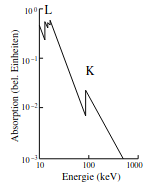
\includegraphics{Absorbtionsspektrum.png}
        \caption{Absorptionsspektrum}
        \label{fig:rechtschreifehler}
      \end{figure}
    Wie in Abbildung \ref{fig:rechtschreifehler} dargestellt, sinkt der Absorbtionskoeffizient bei steigender Energie.
    Unterbrochen wird diese Kurve von sprunghaften Anstiegen, die genau dann auftreten, wenn 
    die Photonenenergie gerade größer als die Bindungsenergie eines Elektron auf einer Schale ist.
    Diese Unstetigkeiten werden nach den jeweiligen Schalen als K-, L-, ... Absorbtionskante
    bezeichnet. Die Bindungsenergie $E_{n,j}$ auf den Schalen kann mittels der 
    Sommerfeldschen Feinstrukturformel
    \begin{equation}
        E_{n, j}=-R_{\inf}(z_{eff}^2 \cdot \dfrac{1}{n^2} + \alpha^2z_{eff}^4 \dfrac{1}{n^3}
        (\dfrac{1}{j+1/2}-\dfrac{3}{4n}))
    \end{equation}
    bestimmt werden. Dabei ist $R_{\inf}$ die Rydbergenergie, $z_{eff}$ die effektive
    Kernladungszahl, $\alpha$ die sommerfeldsche Feinstrukturkonstante, n die Hauptquantenzahl
    und j der Gesamtdrehimpuls des betrachteten Elektrons. In der K-Schale ergibt sich also
    für die Abschirmkonstante 
    \begin{equation}
        \sigma_K = Z - \sqrt{\dfrac{E_K}{R_{\inf}}-\dfrac{\alpha^2 Z^4}{4}}.
        \label{eqn:sigma}
    \end{equation}
    Die Abschirmkonstante für die L-Schale kann durch 
    \begin{equation}
        \sigma_L=Z-(\dfrac{4}{\alpha} \sqrt{\dfrac{\Delta E_L}{R_{\inf}}}-\dfrac{5 \Delta E_L}
        {R_{\inf}})^{1/2} (1+\dfrac{19}{32}\alpha^2 \dfrac{\Delta E_L}{R_{\inf}})^{1/2}
    \end{equation}
    berechnet werden, wobei die Energiedifferenz $\Delta E_L = E_{L_{11}} - E_{L_{111}}$ zwischen 
    $L_{11}$ und $L_{111}$-Kante verwendet wird, da die $L_1$ und $L_{11}$-Kante in diesem
    Versuch nicht bestimmt werden können.

\subsection{Bragg'sche Reflexion}
    Um die Energie bzw die Wellenlänge der Röntgenstrahlung zu bestimmen, wird der Effekt der Braggschen 
    Reflexion verwendet. Denn fällt Röntgenstrahlung auf ein dreidimensionales Gitter
    und wird dort gebeugt, interferieren die ausfallenden Röntgenstrahlen. Ist die 
    Gitterkonstante des verwendeten Materials bekannt, so kann die Wellenlänge durch
    die Beziehung $2 d \sin{\theta}=n \lambda$ bestimmt werden, wobei $\theta$ Glanzwinkel
    und n die Beugungsordnungs ist.